\documentclass{exam}

\usepackage{units} 
\usepackage{xfrac} 
\usepackage[fleqn]{amsmath}
\usepackage{cancel}
\usepackage{float}
\usepackage{mdwlist}
\usepackage{booktabs}
\usepackage{cancel}
\usepackage{polynom}
\usepackage{caption}
\usepackage{fullpage}
\usepackage{comment}
\usepackage{enumerate}
\usepackage{graphicx}

\newcommand{\degree}{\ensuremath{^\circ}} 
\everymath{\displaystyle}

% \printanswers

\ifprintanswers 
  \usepackage{2in1, lscape} 
\fi

\author{}
\date{January 22, 2014}
\title{Statistics \\ Homework One}

\begin{document}

  \maketitle
  \section{Chapter One Homework}

  \begin{itemize*}
    \item read Chapter 1 
    \item answer the questions in ``Check Your Skills'' and check the answers in the back of the book
    \item hand in exercises 23-24, 26, 28, 30-32, 34, 39-41
  \end{itemize*}

  \ifprintanswers
    \section{Chapter 1}
    \begin{description}
      \item[23]
        \begin{parts}
          \part categorical
          \part categorical
          \part quantitative
          \part categorical
          \part quantitative
        \end{parts}

      \item[24]
        \begin{parts}
          \part David Ortiz, Laynce Nix, Antonio Perez, Mike Piazza, and Scott Rolen
          \part team, position, age, height, weight, salary
          \part years, feet and inches, pounds, dollars
        \end{parts}

      \pagebreak

      \item[26]
        To create a pie chart, you would also need to know the number of deaths from all other causes.

        \begin{figure}[H]
          \centering
          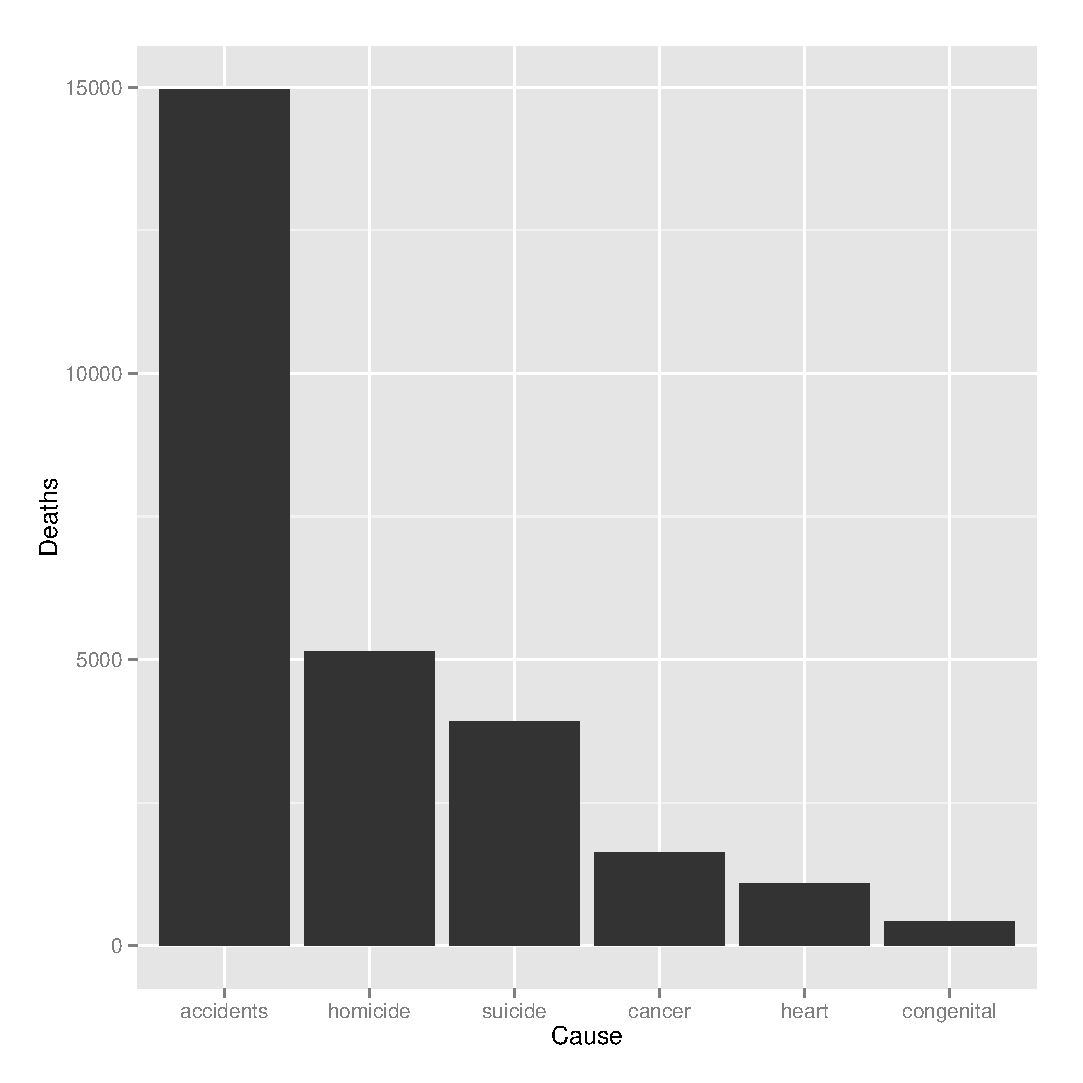
\includegraphics[scale = 0.7]{ex26.eps}
          \caption{Exercise 26}
        \end{figure}

      \item[28]
        \begin{parts}
          \part
            \begin{figure}[H]
              \centering
              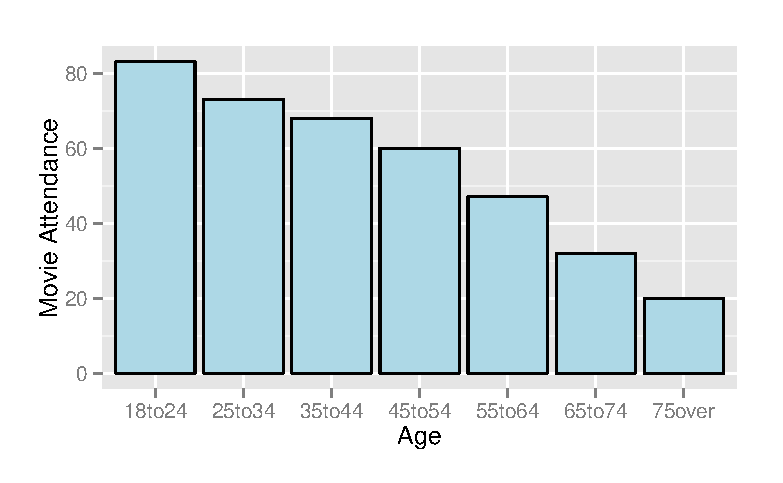
\includegraphics[scale = 0.7]{ex28.eps}
              \caption{Exercise 28}
            \end{figure}

            The main feature of the data is that people watch fewer movies as they get older.

          \part no--the graph shows the percentage of each age group, not percentages of a single total number of people

          \part To answer this question you would need to know how many are in each age group.
        \end{parts}

      \item[30]
        \begin{parts}
          \part
            \begin{itemize*}
              \item The center is around 2 servings--about half the girls eat 2 or fewer servings and about half the
                girls eat more than two servings.

              \item The data is right-skewed.  
            
              \item The spread is from 0 servings to 8 servings.
            \end{itemize*}

          \part 26 out of 74 or 30\% eat less than 2 servings per day
        \end{parts}

      \item[31]
        \begin{parts}
          \part Ignoring the outliers, the shape looks symmetric.

          \part The center seems to be around 2\%.

          \part The smallest return was around -12\% and the largest return was around 14\%.

          \part About a third of the months had a return less than zero.
        \end{parts}

      \item[32]
        \begin{enumerate}
          \item Graph b and graph c both have two choices.  The number of females/males is probably more even than the
            number of left handed/right handed, so graph c is the female/male graph.

          \item graph b

          \item Graph d is evenly distributed around some average number, so this is probably the height.

          \item Graph a shows a bunch of people who don't study at all, with gradually diminishing numbers of people who
            study more hours per night.
        \end{enumerate}

      \item[34]
        \begin{parts}
          \part Since the states have varying numbers of people, it's more interesting to know the ratio of doctors to
          people than the total number of doctors.

          \part 
            \begin{figure}[H]
              \centering
              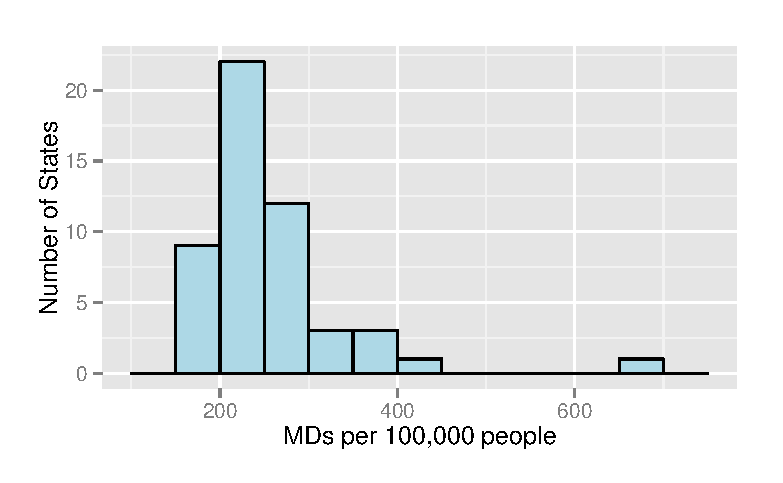
\includegraphics[scale = 0.7]{ex34.eps}
              \caption{Exercise 34}
            \end{figure}

            The histogram is right-skewed with a center around 230.  Washington DC is an outlier, probably because
            it is a city instead of a state.

        \end{parts}

      \item[39]
        \begin{parts}
          \part You would expect the categories with the most drivers to have the most accidents, regardless of any
          effect pot might have on the accident rate.  

          \part 
            \begin{figure}[H]
              \centering
              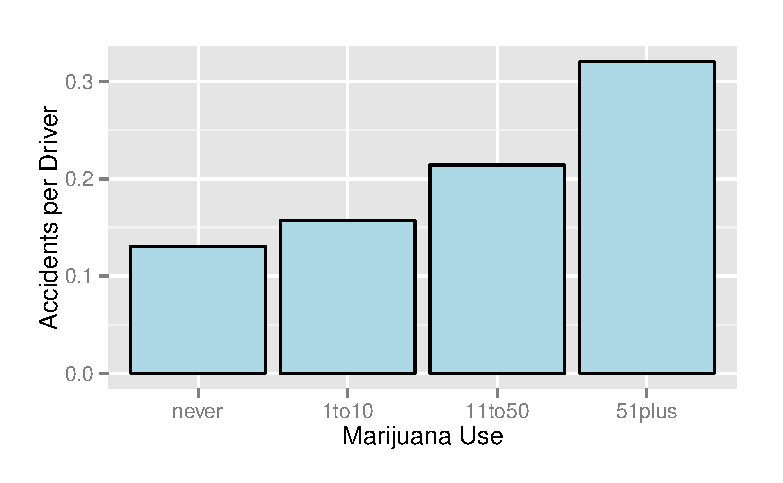
\includegraphics[scale = 0.7]{ex39.eps}
              \caption{Exercise 39}
            \end{figure}

        \end{parts}

      \item[40]
        Most coins you would find would probably have been made in the last decade.  However, coins have a long life, so
        you might find a few coins which are 40 or 50 years old.

      \item[41]
        The important points are:
        \begin{itemize*}
          \item Toyota is consistently better than GM, but the gap has narrowed slightly since 1998.
          \item Toyota improved substantially between 1998 and 2000 and has been relatively constant since then.
          \item GM improved substantially between 1998 and 2002 and has been relatively constant since then.
        \end{itemize*}

        \begin{figure}[H]
          \centering
          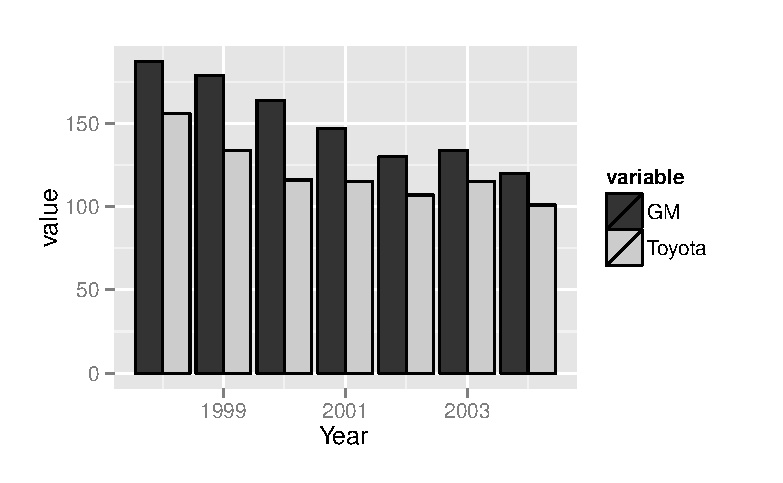
\includegraphics[scale = 0.7]{ex41.eps}
          \caption{Exercise 41}
        \end{figure}

      \item[41]
        In each year, the prices are highest around July and lowest around January.  There is a long term year over year increase in
        the prices.

      \item[44]
        \begin{parts}
          \part
            The center is around 10.  About half the years had less than 10 attacks and about half the years had 10 or more
            attacks.  The data is right skewed--there are a few years with more than 20 attacks and, of course, no years
            with less than zero attacks.

            \begin{figure}[H]
              \centering
              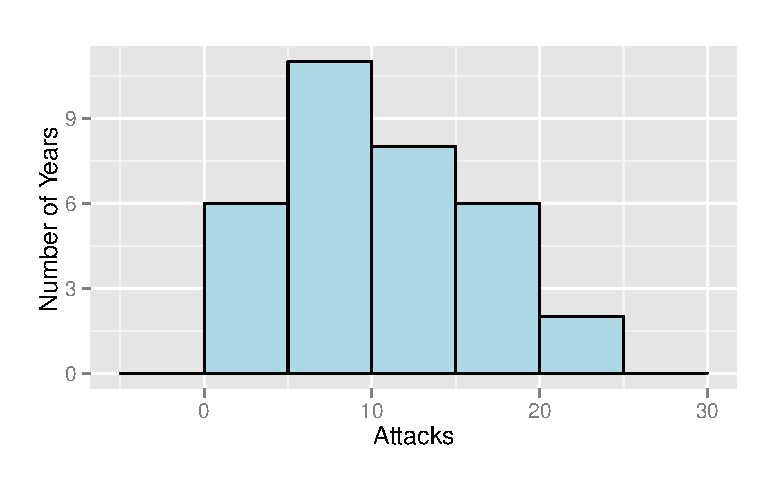
\includegraphics[scale = 0.7]{ex44Histogram.eps}
              \caption{Attacks Histogram}
            \end{figure}

          \part
            There were 6 years with 0-4 attacks but they all occurred before 1986.  There were 15 years with more than 10
            attacks, and they all occurred after 1986.  If you are interested in what's likely to happen in 2006, you should
            pay attention to the more recent numbers and ignore the data from 20 years ago.

            \begin{figure}[H]
              \centering
              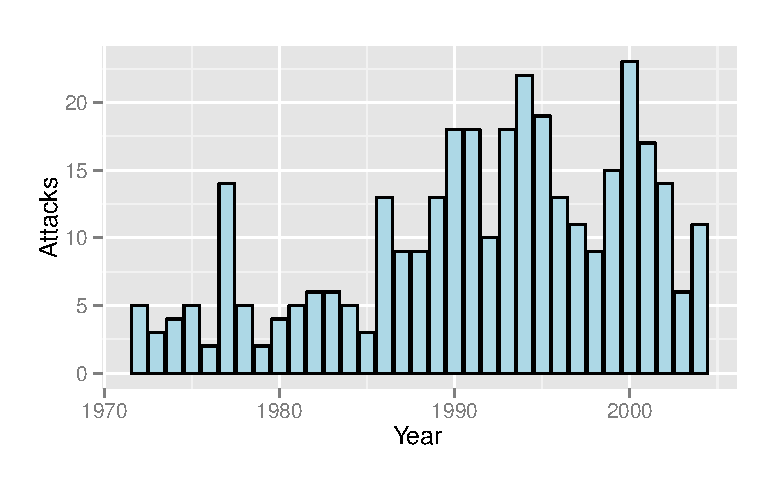
\includegraphics[scale = 0.7]{ex44Time.eps}
              \caption{Attacks by Time}
            \end{figure}
        \end{parts}


    \end{description}

  \else
    \vspace{11 cm}
    \begin{quote}
      \begin{em}
        Even voting for the right is doing nothing for it. It is only expressing to men feebly your desire that it
        should prevail. 
        % A wise man will not leave the right to the mercy of chance, nor wish it to prevail through the power of the
        % majority. There is but little virtue in the action of masses of men. When the majority shall at length vote for
        % the abolition of slavery, it will be because they are indifferent to slavery, or because there is but little
        % slavery left to be abolished by their vote. 
      \end{em}
    \end{quote}
    \hspace{1 cm} --Henry David Thoreau
  \fi

\end{document}

